In the first stage in our offline training, to initialize the weights for reinforcement learning of the policy network, a 13-layer supervised learning (SL) policy network was trained using a randomly sampled dataset (state-action pairs) from 30 million expert human moves (KGS Go Server). The SL policy network $p_\sigma(a|s)$ takes an input $s$ (Extended Table 2 in\cite{b12}), alternates between convolutional layers and rectifier nonlinearities, and outputs a probability distribution over all legal moves $a$ using a final softmax layer. The policy network was trained using stochastic gradient ascent to maximize the likelihood of the human move $a$ selected in state $s$,
\begin{equation}
    \nabla \sigma \propto \frac{\partial \log p_\sigma (a|s)}{\partial \sigma}.
\end{equation}
The network predicted expert moves on a held-out test set with an accuracy of 57.0\% using all input features and 55.7\% using only raw board position and move history as inputs. Minor improvements in accuracy led to significant improvements in playing strength (cf. Fig.~\ref{SL_strength}); more extensive networks achieve better accuracy but are slower to evaluate during search (see Extended Table 3 in\cite{b12} for accuracies of these networks).

\begin{figure}[t]
\centerline{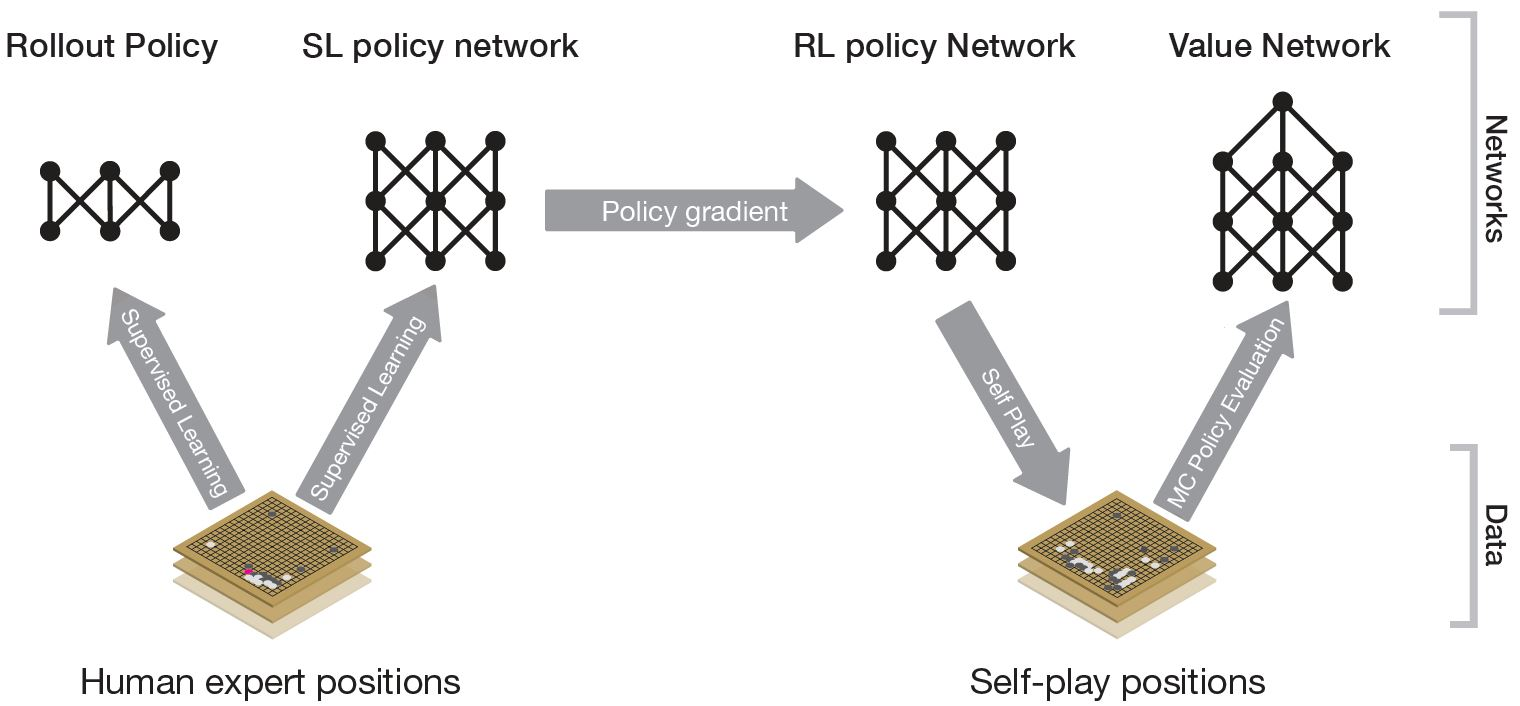
\includegraphics[width = \columnwidth]{ML_pipeline_3.jpg}}
\caption{Machine learning training pipeline of AlphaGo\cite{b12}}
\label{ML_pipe_1}
\end{figure} 

\begin{figure}[b]
\centerline{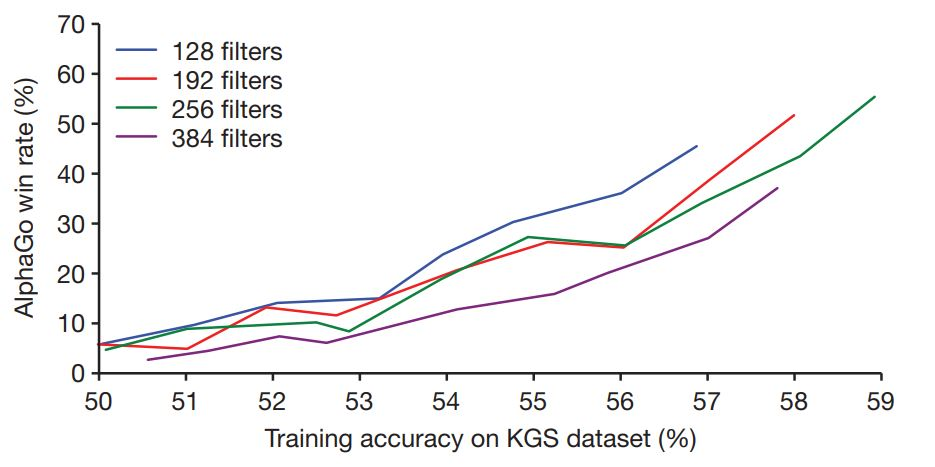
\includegraphics[width = 0.8\columnwidth]{Sl_strength.JPG}}
\caption{Strength of supervised learning policy network\cite{b12}}
\label{SL_strength}
\end{figure}


% \begin{figure*}[t]
% \centerline{\includegraphics[width = 5in]{ML_pipeline_2.jpg}}
% \caption{Offline machine learning training pipeline of AlphaGo}
% \label{ML_pipe}
% \end{figure*}

% \begin{table*}[]
%     \centering
%     \begin{tabular}{c|c}
%          &  \\
%          & 
%     \end{tabular}
%     \caption{Caption}
%     \label{tab:my_label}
% \end{table*}